\documentclass[12pt]{article}
\usepackage[utf8]{inputenc}
\usepackage{hyperref}
\usepackage{listings}
\usepackage{xcolor}
\usepackage{geometry}
\usepackage{graphicx} % For including graphics
\usepackage{minted} % For advanced code listings
\usepackage{listings-solidity}  % Include Solidity highlighting
\usepackage{amsmath, amssymb, amsfonts} % For mathematical equations


% Define a custom minted style (optional)
\usemintedstyle{colorful} % You can choose from various styles like 'monokai', 'tango', 'colorful', etc.

% Custom color setup
\definecolor{bashtextcolor}{RGB}{0, 0, 0} % Define black color

% Define a new command for inline code using minted
\newcommand{\codeinline}[1]{\mintinline{text}{#1}}

\geometry{a4paper, margin=1in}

\title{Smart Contracts Exercise 08: \\ Maximal Extractable Value}
\author{}
\date{}

% Define a new command for inline code with a dark background
\newcommand{\codeblack}[1]{%
  \texttt{\colorbox{black!7}{\textcolor{black}{#1}}}%
}

% Define a new command for inline code with a dark background
\newcommand{\codegrey}[1]{%
  \texttt{\colorbox{black!4}{\textcolor{black}{#1}}}%
}

% Define custom colors (optional)
\definecolor{myURLColor}{RGB}{0, 102, 204} % Example: A shade of blue

\hypersetup{
    colorlinks=true,        % Enable colored links
    linkcolor=blue,         % Color for internal links (e.g., \ref, \cite)
    citecolor=blue,         % Color for citations
    filecolor=magenta,      % Color for file links
    urlcolor=myURLColor     % Color for external URLs
}

% Define a style for code listings
\lstdefinestyle{mystyle}{
    backgroundcolor=\color{lightgray!20},   
    commentstyle=\color{green!50!black},
    keywordstyle=\color{blue},
    numberstyle=\tiny\color{gray},
    stringstyle=\color{red},
    basicstyle=\ttfamily\footnotesize,
    breakatwhitespace=false,         
    breaklines=true,                 
    captionpos=b,                    
    keepspaces=true,                 
    numbers=left,                    
    numbersep=5pt,                  
    showspaces=false,                
    showstringspaces=false,
    showtabs=false,                  
    tabsize=2
}

\lstset{style=mystyle}
% Adding package for header and footer
\usepackage{fancyhdr}
\pagestyle{fancy}

% Define header and footer
\fancyhf{} % Clear current settings
\fancyhead[L]{Smart Contracts Exercise 08} % Left header
\fancyhead[R]{\thepage} % Right header with page number

\renewcommand{\headrulewidth}{0.4pt} % Line below header
% \renewcommand{\footrulewidth}{0.4pt} % Line above footer

\begin{document}

\maketitle
\section{Introduction}

We first encountered frontrunning in Exercise 3: ERC20 - CTUToken. Frontrunning falls under the more general term known as MEV - Maximal Extractable Value. MEV has become a very important topic for Ethereum that needs to be addressed. In this exercise, we will examine this phenomenon in more detail. We'll explore additional MEV techniques and examples, such as DEX arbitrage, liquidations, sandwich trading, and more. An important topic of the exercise will also be calculating transaction fees, gas, and understanding EIP-1559. In the practical exercises, you will try frontrunning an NFT auction and executing a sandwich attack on a DEX yourself. Finally, we'll look at how MEV is being solved today and introduce terms such as Proposer-Builder Separation and Builder APIs.

\subsection*{Project Setup}

You have two options for working with this exercise: using a Docker container or local installation. Choose the option that best fits your preferences.

\subsection{Using Docker with VS Code}

This option uses Docker to create a development environment with all the necessary tools and dependencies pre-installed.

\subsubsection*{Prerequisites:}

\begin{itemize}
    \item \textbf{\href{https://www.docker.com/products/docker-desktop}{Docker}} - A platform for developing, shipping, and running applications in containers.
    \item \textbf{\href{https://code.visualstudio.com/}{Visual Studio Code}} - A lightweight but powerful source code editor.
    \item \textbf{\href{https://marketplace.visualstudio.com/items?itemName=ms-vscode-remote.remote-containers}{Dev Containers}} - An extension to VS Code that lets you use a Docker container as a full-featured development environment.
\end{itemize}

\subsubsection*{Setting Up the Project:}

\begin{enumerate}
  \item Visit the following \href{https://github.com/radovluk/Smart-Contract-Exercise/tree/main/08-Maximal-Extractable-Value/task/task-code}{GitHub repository} and clone it to your local machine.
  \item Open the repository folder in VS Code.
  \item When prompted, click ``Reopen in Container'' or use the command palette (F1) and run \codegrey{Dev Containers: Reopen in Container}.
\end{enumerate}

\subsection{Local Setup}

If you prefer working directly on your machine without Docker, you can set up the development environment locally.

\subsubsection*{Prerequisites}
\begin{itemize}
    \item \textbf{Node.js}: \url{https://nodejs.org/en/} - An open-source, cross-platform, back-end JavaScript runtime environment that runs on the V8 engine and executes JavaScript code outside a web browser.
    \item \textbf{NPM}: Node Package Manager, which comes with Node.js.
\end{itemize}

\noindent
Open your terminal and run the following commands to verify the installations:

\begin{minted}[bgcolor=gray!5, fontsize=\footnotesize]{bash}
$ node -v
$ npm -v
\end{minted}

Both commands should return the installed version numbers of Node.js and NPM respectively. Node.js provides the runtime environment required to execute JavaScript-based tools like Hardhat, while NPM is used to manage the packages and dependencies needed for development.

\subsubsection*{Setting Up the Project}

\begin{enumerate}
    \item Visit the following \href{https://github.com/radovluk/Smart-Contract-Exercise/tree/main/08-Maximal-Extractable-Value/task/task-code}{GitHub repository} and clone it to your local machine.
    \item Open a terminal and navigate to the project directory.
    \item Install the project dependencies by running \codegrey{npm install}.
\end{enumerate}

\section{Maximal Extractable Value (MEV)}

MEV stands for Maximal Extractable Value, which refers to the maximum value that can be extracted during block production in addition to the standard block rewards and gas fees. This value can be extracted by adding transactions to a block, removing transactions from it, or changing the order of transactions within the block. Originally, the acronym stood for ``Miner Extractable Value,'' but since \href{https://ethereum.org/en/roadmap/merge/}{the Merge} replaced miners with validators, it's now known as ``Maximal Extractable Value''.

\subsection*{Types of MEV}

Several types of MEV extraction can be identified:

\begin{enumerate}
  \item \textbf{Frontrunning}: An attacker observes a pending transaction in the mempool and submits their own transaction to be included in the block before the original transaction.
  \item \textbf{Backrunning}: An attacker observes a pending transaction in the mempool and submits their own transaction to be included in the block immediately after the original transaction.
  \item \textbf{Sandwich Attack}: An attacker places two transactions around the victim's transaction - one before and one after.
  \item \textbf{Transaction Censorship}: An attacker omits a transaction from the block to prevent it from being executed.
\end{enumerate}

\begin{figure}[H]
  \centering
  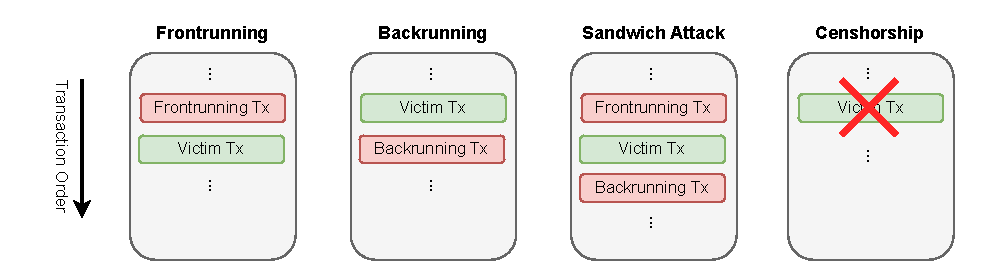
\includegraphics[width=1\textwidth]{MEV.pdf}
  % \caption{Frontrunning Attack}
  \label{fig:sandwich}
\end{figure}

\noindent
To better understand why these techniques are profitable for attackers, let's examine some specific examples:

\subsubsection*{DEX Arbitrage} If two DEXes offer tokens at different prices, someone can include a transaction in a block that buys tokens on one DEX and sells them at a higher price on another DEX. In this situation, the block creator can exploit this opportunity to profit from the arbitrage. Here's an \href{https://etherscan.io/tx/0x5e1657ef0e9be9bc72efefe59a2528d0d730d478cfc9e6cdd09af9f997bb3ef4}{example of such transaction}.

\subsubsection*{Sandwich Attack}
If someone wants to exchange a large amount of a specific token on a DEX, an attacker can add transactions that buy tokens before the large transaction and sell them afterward. Thanks to how DEXes set prices using the constant product formula ($x \cdot y = k$), this approach can be profitable. See an example of \href{https://eigenphi.io/mev/ethereum/tx/0x90204899500606f717cacd223fc27b2be0e017032c7f41986cfb094e686630b4}{such an attack}. The process is detailed in Table~\ref{tab:sandwich-attack} and illustrated in Figure~\ref{fig:sandwich}.

\begin{figure}[H]
  \centering
  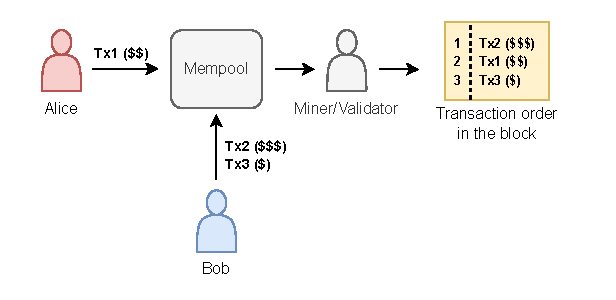
\includegraphics[width=0.75\textwidth]{sandwich.pdf}
  \caption{Sandwich Attack visualization showing how transactions are ordered in the mempool and block.}
  \label{fig:sandwich}
\end{figure}

\begin{table}[h]
  \centering
  \footnotesize
  \begin{tabular}{|p{0.05\textwidth}|p{0.2\textwidth}|p{0.6\textwidth}|}
  \hline
  \textbf{Step} & \textbf{Action} & \textbf{Description} \\
  \hline
  1 & Alice creates transaction & Alice submits transaction Tx1 (\$\$) to the mempool to swap a large amount of tokens on a DEX. \\
  \hline
  2 & Bob monitors mempool & Bob identifies Alice's pending transaction as an opportunity for a sandwich attack. \\
  \hline
  3 & Bob creates frontrun & Bob submits transaction Tx2 (\$\$\$) with higher gas fees to buy the same tokens before Alice's swap executes. \\
  \hline
  4 & The token price increases & After Bob's purchase, token price increases according to $P_{\text{new}} = \frac{y - \Delta y}{x + \Delta x}$ where $\Delta x$ is Bob's input and $\Delta y$ is tokens received. \\
  \hline
  5 & Alice's transaction executes & Alice's swap executes at worse price conditions due to Bob's prior purchase, receiving fewer tokens than expected. \\
  \hline
  6 & Token price increases further & Alice's large swap further increases the token price due to the constant product formula, making Bob's tokens worth more. \\
  \hline
  7 & Bob executes backrun & Bob's transaction Tx3 (\$) sells the tokens at the higher price caused by Alice's large swap. \\
  \hline
  8 & Bob profits & Bob profits from the price difference: $\text{Profit} = \text{Sell proceeds} - \text{Purchase cost} - \text{Gas fees}$. \\
  \hline
  9 & Price impact on Alice & Alice experiences negative price impact, receiving fewer tokens than expected in a fair market. \\
  \hline
  \end{tabular}
  \caption{Sandwich Attack Mechanism on a DEX. The attack exploits the AMM pricing formula and transaction ordering. For visual representation, see Figure~\ref{fig:sandwich}.}
  \label{tab:sandwich-attack}
\end{table}

\subsubsection*{Liquidations} When borrowers in lending protocols fall below required collateralization ratios, their positions become eligible for liquidation. Block producers can prioritize their own liquidation transactions, allowing them to claim the liquidation rewards and discounted collateral before other participants. This gives them an advantage in capturing value from distressed positions. See \href{https://eigenphi.io/mev/ethereum/liquidation}{examples of such transactions}.

\subsubsection*{Other MEVs}
MEV opportunities are derived from smart contracts and their functionalities. Consider, for example, the auction from the previous exercise. If the block creator is interested in the auctioned item, they can simply add their transaction at the end of the auction, placing it before the transaction that ends the auction.

See also this example where a MEV searcher purchased every single \href{https://cryptopunks.app/}{Cryptopunk} at the floor price for 7 million USD: \href{https://etherscan.io/address/0x650dCdEB6ecF05aE3CAF30A70966E2F395d5E9E5}{Searcher's address}.

\subsubsection*{Generalized frontrunning}

Rather than developing complicated algorithms, it's possible to simply simulate transactions in the mempool. If a transaction results in profit, a frontrunner can copy the potentially profitable transaction and replace the address with their own. If the transaction still generates profit with the modified address, the attacker can include it in the block and claim the profit for themselves.

\subsection{MEV Threat and Solutions}

MEV bots attempting to include their MEV transactions in blocks have led to network congestion and increased transaction fees for regular users. MEV extraction could eventually lead to gradual centralization of staking pools, as large pools will have more financial resources to develop sophisticated algorithms to extract MEV. To address these MEV problems, solutions have been proposed: \href{https://ethereum.org/en/developers/docs/mev/#proposer-builder-separation}{Proposer-builder separation} and \href{https://ethereum.org/en/developers/docs/mev/#builder-api}{Builder APIs}. In proposer-builder separation, validators remain responsible for proposing new blocks, but a new entity of specialized builders has emerged who search for MEV opportunities and offer constructed blocks to validators. This reduces the risk of validator centralization. For smart contract developers, it's important to always keep MEV risks in mind and mitigate them during application design when possible.

\medskip
\noindent
More about MEV:
\begin{itemize}
  \item \textbf{Read}: \href{https://ethereum.org/en/developers/docs/mev/}{Maximal extractable value (MEV)}
  \item \textbf{Animated Video}: \href{https://www.youtube.com/watch?v=F9IuBZGseFQ}{Decoding MEV: Past, Present, Future}
  \item \textbf{MEV Real Time Detection}: \href{https://eigenphi.io/}{https://eigenphi.io}
  \item \textbf{Read}: \href{https://www.flashbots.net/}{Flashbots research blog}
  \item \textbf{Block Building Visualisation}: \href{https://payload.de/data/}{https://payload.de/data}
  \item \textbf{MEV Boost Dashboard}: \href{https://mevboost.pics/}{https://mevboost.pics}
\end{itemize}

\section{Gas and Fees}

\textbf{Gas} is a unit that measures the computational effort required to execute a specific operation on the Ethereum network. The \textbf{gas fee} is the amount of gas used for a particular operation multiplied by the price per unit of gas. The costs of individual operations can be viewed at \href{https://ethereum.org/en/developers/docs/evm/opcodes/}{EVM Opcodes}.

\subsubsection*{Gas Price Determination}

Previously, users would specify a \codegrey{gasprice} which operated as a simple auction system - higher gas price meant higher priority. However, this solution had several drawbacks, so Ethereum transitioned to a new transaction fee mechanism according to \href{https://eips.ethereum.org/EIPS/eip-1559}{EIP-1559}. Instead of users trying to estimate how much to bid, the Ethereum protocol now determines a \textbf{base fee} that must be paid for a transaction to be included in a block. This base fee dynamically increases or decreases by a maximum of 12.5\% with each block. Each block has a limit of 30 million gas, but the target is 15 million:

\begin{itemize}
    \item If a block used less than 15 million gas, the base fee decreases
    \item If the block was congested, the base fee increases
\end{itemize}

\noindent
The base fee doesn't go to validators but is \textbf{burned} (removed from circulation). EIP-1559 also introduced a \textbf{priority fee}, which goes directly to validators as a tip to incentivize them to include the transaction in a block. Transaction initiators can also specify a \textbf{maximum gas price} (\codegrey{max fee}) they're willing to pay per unit of gas. The actual fee per gas paid by a transaction is calculated as:

\begin{equation}
\text{gasprice} = \min(\text{base fee} + \text{priority fee}, \text{max fee})
\end{equation}

Where:
\begin{itemize}
    \item \codegrey{base fee} is burned (removed from circulation)
    \item \codegrey{priority fee} (or tip) goes to the validator as an incentive
    \item If \codegrey{base fee} + \codegrey{priority fee} \verb|>| \codegrey{max fee}, the priority fee is reduced to stay below the max fee
\end{itemize}

\noindent
Any difference between the max fee and the base fee is refunded to the transaction initiator. The total fee paid for a transaction is:

\begin{equation}
\text{transaction fee} = \text{gas used} \times \text{gasprice}
\end{equation}

\medskip
\noindent
More about Gas and Fees:
\begin{itemize}
  \item \textbf{Read}: \href{https://ethereum.org/en/developers/docs/gas/}{Gas and Fees}
  \item \textbf{Gas tracker}: \href{https://etherscan.io/gastracker}{https://etherscan.io/gastracker}
  \item \textbf{Video}: \href{https://www.youtube.com/watch?v=MGemhK9t44Q}{Can ETH Become DEFLATIONARY? EIP 1559 Explained}
\end{itemize}

\pagebreak
\section{Task}

\subsection*{Task 1: NFT Auction Frontrunning}
Another rare NFT from the FEL Student Collection is up for auction - specifically, a student from the OES program caught sleepwalking with a laptop (apparently a common occurrence during exam season). This time the auction is well-protected against DoS attacks and fully implements the push-over-pull pattern from the previous exercise. The bidding has already reached 1.5 ETH. You don't want to place bids until the last possible moment to avoid being outbid. You've been monitoring the public mempool, waiting for the event organizer to call the \codegrey{endAuction()} function so you can be the final bidder. 

With 1.51 ETH in your wallet and a strong desire for this NFT, you're watching closely for your chance to place a bid just before the auction officially ends...

\begin{figure}[H]
  \centering
  \begin{minipage}{0.3\textwidth}
    
\includegraphics[width=\textwidth]{NFTs/oes-student-nft.pdf}
  \end{minipage}
\end{figure}

\medskip
\noindent
\textbf{Your Mission}:
\begin{itemize}
    \item Monitor the mempool for the \codegrey{endAuction()} transaction
    \item Gain the OES student NFT
\end{itemize}

\noindent
Code your solution in the \texttt{test/NFTAuction.js} file. Use the player account only. See \href{https://docs.ethers.org/v6/api/transaction/\#Transaction}{Ethers v6 transaction documentation} to learn how to specify transaction fees. Verify your solution by running:

\begin{minted}[bgcolor=gray!5, fontsize=\footnotesize]{bash}
$ npm run auction
\end{minted}

\noindent
Files that are relevant for this challenge:
\begin{itemize}
\item test/\textbf{NFTAuction.js}: The test file where you should code your solution.
\item contracts/\textbf{NFTAuction.sol}: The improved auction contract.
\item contracts/\textbf{FELStudentNFT.sol}: The NFT collection contract.
\end{itemize}

\subsection*{Task 2: Sandwich Attack on a DEX}

You've been monitoring the mempool and spotted a juicy opportunity: someone (let's call them ``Innocent Victim'') is about to swap a massive 20 ETH for USDC tokens on SimpleDEX. With your knowledge of DeFi and MEV, you realize this is a perfect opportunity for a sandwich attack.

You have 15 ETH at your disposal, and your blockchain professor would be so proud to see you apply your knowledge in real life (or maybe not...).

\medskip
\noindent
\textbf{Your Mission}:
\begin{itemize}
  \item Execute a sandwich attack on the victim's transaction
  \item Make a profit of at least 1 ETH from this MEV extraction
\end{itemize}

\noindent
Code your solution in the \texttt{test/SandwichAttack.js} file. Use the player account for your transactions. Verify your solution by running:

\begin{minted}[bgcolor=gray!5, fontsize=\footnotesize]{bash}
$ npm run sandwich
\end{minted}

\noindent
Files that are relevant for this challenge:
\begin{itemize}
\item test/\textbf{SandwichAttack.js}: The test file where you should code your solution.
\item contracts/\textbf{SimpleDEX.sol}: A decentralized exchange with a one liquidity pool containing 500 ETH and 1,000,000 USDC.
\item contracts/\textbf{USDCToken.sol}: An ERC20 token representing simplified version of USDC.
\end{itemize}

\end{document}